\documentclass[twoside]{book}

% Packages required by doxygen
\usepackage{fixltx2e}
\usepackage{calc}
\usepackage{doxygen}
\usepackage[export]{adjustbox} % also loads graphicx
\usepackage{graphicx}
\usepackage[utf8]{inputenc}
\usepackage{makeidx}
\usepackage{multicol}
\usepackage{multirow}
\PassOptionsToPackage{warn}{textcomp}
\usepackage{textcomp}
\usepackage[nointegrals]{wasysym}
\usepackage[table]{xcolor}

% Font selection
\usepackage[T1]{fontenc}
\usepackage[scaled=.90]{helvet}
\usepackage{courier}
\usepackage{amssymb}
\usepackage{sectsty}
\renewcommand{\familydefault}{\sfdefault}
\allsectionsfont{%
  \fontseries{bc}\selectfont%
  \color{darkgray}%
}
\renewcommand{\DoxyLabelFont}{%
  \fontseries{bc}\selectfont%
  \color{darkgray}%
}
\newcommand{\+}{\discretionary{\mbox{\scriptsize$\hookleftarrow$}}{}{}}

% Page & text layout
\usepackage{geometry}
\geometry{%
  a4paper,%
  top=2.5cm,%
  bottom=2.5cm,%
  left=2.5cm,%
  right=2.5cm%
}
\tolerance=750
\hfuzz=15pt
\hbadness=750
\setlength{\emergencystretch}{15pt}
\setlength{\parindent}{0cm}
\setlength{\parskip}{3ex plus 2ex minus 2ex}
\makeatletter
\renewcommand{\paragraph}{%
  \@startsection{paragraph}{4}{0ex}{-1.0ex}{1.0ex}{%
    \normalfont\normalsize\bfseries\SS@parafont%
  }%
}
\renewcommand{\subparagraph}{%
  \@startsection{subparagraph}{5}{0ex}{-1.0ex}{1.0ex}{%
    \normalfont\normalsize\bfseries\SS@subparafont%
  }%
}
\makeatother

% Headers & footers
\usepackage{fancyhdr}
\pagestyle{fancyplain}
\fancyhead[LE]{\fancyplain{}{\bfseries\thepage}}
\fancyhead[CE]{\fancyplain{}{}}
\fancyhead[RE]{\fancyplain{}{\bfseries\leftmark}}
\fancyhead[LO]{\fancyplain{}{\bfseries\rightmark}}
\fancyhead[CO]{\fancyplain{}{}}
\fancyhead[RO]{\fancyplain{}{\bfseries\thepage}}
\fancyfoot[LE]{\fancyplain{}{}}
\fancyfoot[CE]{\fancyplain{}{}}
\fancyfoot[RE]{\fancyplain{}{\bfseries\scriptsize Generated by Doxygen }}
\fancyfoot[LO]{\fancyplain{}{\bfseries\scriptsize Generated by Doxygen }}
\fancyfoot[CO]{\fancyplain{}{}}
\fancyfoot[RO]{\fancyplain{}{}}
\renewcommand{\footrulewidth}{0.4pt}
\renewcommand{\chaptermark}[1]{%
  \markboth{#1}{}%
}
\renewcommand{\sectionmark}[1]{%
  \markright{\thesection\ #1}%
}

% Indices & bibliography
\usepackage{natbib}
\usepackage[titles]{tocloft}
\setcounter{tocdepth}{3}
\setcounter{secnumdepth}{5}
\makeindex

% Hyperlinks (required, but should be loaded last)
\usepackage{ifpdf}
\ifpdf
  \usepackage[pdftex,pagebackref=true]{hyperref}
\else
  \usepackage[ps2pdf,pagebackref=true]{hyperref}
\fi
\hypersetup{%
  colorlinks=true,%
  linkcolor=blue,%
  citecolor=blue,%
  unicode%
}

% Custom commands
\newcommand{\clearemptydoublepage}{%
  \newpage{\pagestyle{empty}\cleardoublepage}%
}

\usepackage{caption}
\captionsetup{labelsep=space,justification=centering,font={bf},singlelinecheck=off,skip=4pt,position=top}

%===== C O N T E N T S =====

\begin{document}

% Titlepage & ToC
\hypersetup{pageanchor=false,
             bookmarksnumbered=true,
             pdfencoding=unicode
            }
\pagenumbering{alph}
\begin{titlepage}
\vspace*{7cm}
\begin{center}%
{\Large btosg }\\
\vspace*{1cm}
{\large Generated by Doxygen 1.8.13}\\
\end{center}
\end{titlepage}
\clearemptydoublepage
\pagenumbering{roman}
\tableofcontents
\clearemptydoublepage
\pagenumbering{arabic}
\hypersetup{pageanchor=true}

%--- Begin generated contents ---
\chapter{R\+E\+A\+D\+ME}
\label{md_README}
\Hypertarget{md_README}
\href{https://travis-ci.org/miguelleitao/btosg}{\tt } \section*{btosg}

A thin abstraction layer to integrate {\bfseries Bullet} and {\bfseries Open\+Scene\+Graph}.

\subsubsection*{Description}

{\bfseries btosg} is aimed to ease building simple visual simulation applications integrating {\bfseries Bullet} and {\bfseries Open\+Scene\+Graph}. {\bfseries btosg} stands on top of these two A\+P\+Is but does not try to hide them. Instead, in order to build a complete application, the programmer is able and usually needs to access directly the data structures from both {\bfseries Bullet} and {\bfseries Open\+Scene\+Graph}. So, the use of {\bfseries btosg} does not avoid the requirement to know and understand their A\+P\+Is.

The use of {\bfseries btosg} can help the programming task because it allows to create and position both the physical and graphics definitions of small objects in one step. It also keeps track of syncronizing the graphics definitions from the state of each physical object.

\subsubsection*{Dependences}

\paragraph*{Open\+Scene\+Graph\+:}


\begin{DoxyItemize}
\item \href{https://github.com/openscenegraph/OpenSceneGraph}{\tt https\+://github.\+com/openscenegraph/\+Open\+Scene\+Graph}
\item \href{http://www.openscenegraph.org/}{\tt http\+://www.\+openscenegraph.\+org/} \paragraph*{Bullet\+:}
\end{DoxyItemize}


\begin{DoxyItemize}
\item \href{https://github.com/bulletphysics/bullet3}{\tt https\+://github.\+com/bulletphysics/bullet3}
\item \href{http://bulletphysics.org/}{\tt http\+://bulletphysics.\+org/}
\end{DoxyItemize}

Dependences can be installed by (assuming Fedora Linux)\+: dnf install bullet openscenegraph-\/osg openscenegraph-\/osg\+Viewer openscenegraph-\/osg\+Sim openscenegraph-\/osg\+DB openscenegraph-\/osg\+GA openscenegraph-\/osg\+Shadow

\subsubsection*{Build}

git clone \href{https://github.com/miguelleitao/btosg.git}{\tt https\+://github.\+com/miguelleitao/btosg.\+git} cd btosg make sudo make install

\subsubsection*{Usage}

Look at provided examples. Prepare your {\itshape application.\+cpp} using \begin{DoxyVerb}#include <btosg.h>
\end{DoxyVerb}


Compile using 
\begin{DoxyPre}
g++ -c `pkg-config --cflags btosg` {\itshape application.cpp}
g++ -o {\itshape application} `pkg-config --libs btosg` {\itshape application.o}
\end{DoxyPre}
 \subsubsection*{Examples}

{\bfseries btosg} is available with some working examples.
\begin{DoxyItemize}
\item {\bfseries ball.\+cpp} implements a simple simulation of a ball with two planes.
\item {\bfseries objects.\+cpp} provides an example for creating a complete object (graphical and physical) from loading an external Wavefront O\+BJ file.
\item {\bfseries car.\+cpp} implements a basic vehicle with four wheels and suspensions. It can be compiled using a Z or Y pointing up vector. Usage instructions are provided in source file.
\end{DoxyItemize}

To compile and try the provided examples do\+: \begin{DoxyVerb}make examples 
./ball
./objects
./carZ
./carY\end{DoxyVerb}
 
\chapter{Hierarchical Index}
\section{Class Hierarchy}
This inheritance list is sorted roughly, but not completely, alphabetically\+:\begin{DoxyCompactList}
\item \contentsline{section}{btosg\+Object}{\pageref{classbtosgObject}}{}
\begin{DoxyCompactList}
\item \contentsline{section}{btosg\+Box}{\pageref{classbtosgBox}}{}
\begin{DoxyCompactList}
\item \contentsline{section}{Block\+Blue}{\pageref{classBlockBlue}}{}
\item \contentsline{section}{Block\+Green}{\pageref{classBlockGreen}}{}
\item \contentsline{section}{Block\+Red}{\pageref{classBlockRed}}{}
\end{DoxyCompactList}
\item \contentsline{section}{btosg\+Cone}{\pageref{classbtosgCone}}{}
\item \contentsline{section}{btosg\+Cylinder}{\pageref{classbtosgCylinder}}{}
\item \contentsline{section}{btosg\+Plane}{\pageref{classbtosgPlane}}{}
\item \contentsline{section}{btosg\+Sphere}{\pageref{classbtosgSphere}}{}
\item \contentsline{section}{btosg\+Vehicle}{\pageref{classbtosgVehicle}}{}
\end{DoxyCompactList}
\item \contentsline{section}{btosg\+World}{\pageref{classbtosgWorld}}{}
\item G\+U\+I\+Event\+Handler\begin{DoxyCompactList}
\item \contentsline{section}{Event\+Handler}{\pageref{classEventHandler}}{}
\end{DoxyCompactList}
\item Projection\begin{DoxyCompactList}
\item \contentsline{section}{btosg\+H\+UD}{\pageref{classbtosgHUD}}{}
\end{DoxyCompactList}
\end{DoxyCompactList}

\chapter{Class Index}
\section{Class List}
Here are the classes, structs, unions and interfaces with brief descriptions\+:\begin{DoxyCompactList}
\item\contentsline{section}{\hyperlink{classBlockBlue}{Block\+Blue} }{\pageref{classBlockBlue}}{}
\item\contentsline{section}{\hyperlink{classBlockGreen}{Block\+Green} }{\pageref{classBlockGreen}}{}
\item\contentsline{section}{\hyperlink{classBlockRed}{Block\+Red} }{\pageref{classBlockRed}}{}
\item\contentsline{section}{\hyperlink{classbtosgBox}{btosg\+Box} }{\pageref{classbtosgBox}}{}
\item\contentsline{section}{\hyperlink{classbtosgCone}{btosg\+Cone} }{\pageref{classbtosgCone}}{}
\item\contentsline{section}{\hyperlink{classbtosgCylinder}{btosg\+Cylinder} }{\pageref{classbtosgCylinder}}{}
\item\contentsline{section}{\hyperlink{classbtosgHUD}{btosg\+H\+UD} }{\pageref{classbtosgHUD}}{}
\item\contentsline{section}{\hyperlink{classbtosgObject}{btosg\+Object} }{\pageref{classbtosgObject}}{}
\item\contentsline{section}{\hyperlink{classbtosgPlane}{btosg\+Plane} }{\pageref{classbtosgPlane}}{}
\item\contentsline{section}{\hyperlink{classbtosgSphere}{btosg\+Sphere} }{\pageref{classbtosgSphere}}{}
\item\contentsline{section}{\hyperlink{classbtosgVehicle}{btosg\+Vehicle} }{\pageref{classbtosgVehicle}}{}
\item\contentsline{section}{\hyperlink{classbtosgWorld}{btosg\+World} }{\pageref{classbtosgWorld}}{}
\item\contentsline{section}{\hyperlink{classEventHandler}{Event\+Handler} }{\pageref{classEventHandler}}{}
\end{DoxyCompactList}

\chapter{Class Documentation}
\hypertarget{classBlockBlue}{}\section{Block\+Blue Class Reference}
\label{classBlockBlue}\index{Block\+Blue@{Block\+Blue}}
Inheritance diagram for Block\+Blue\+:\begin{figure}[H]
\begin{center}
\leavevmode
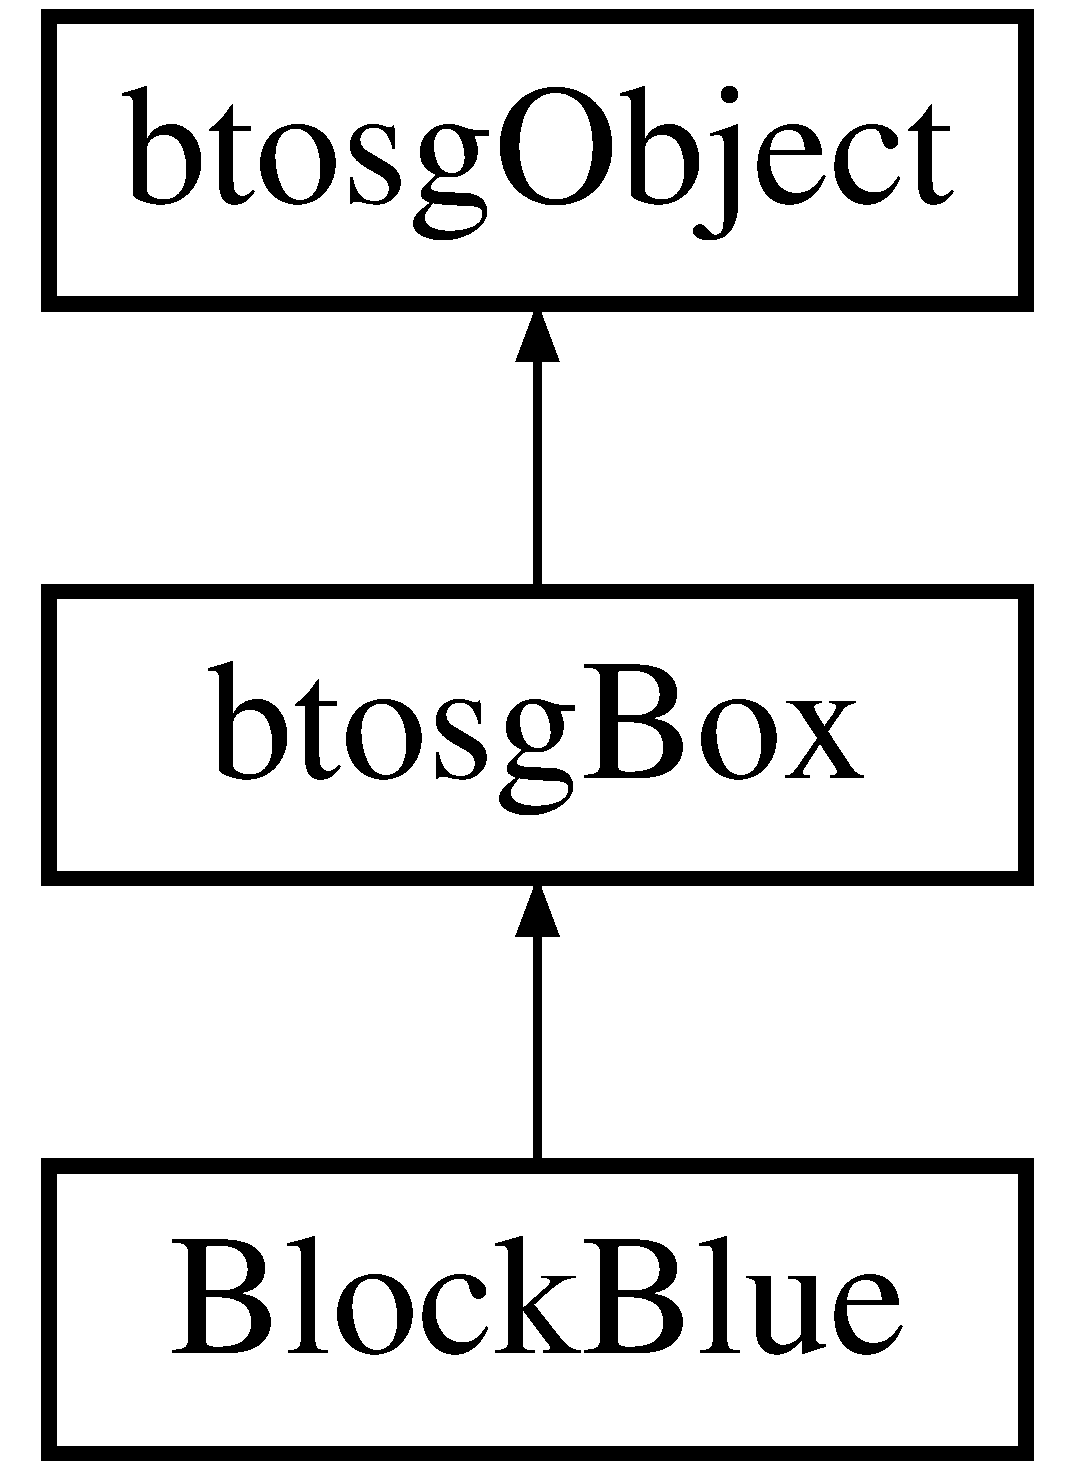
\includegraphics[height=3.000000cm]{classBlockBlue}
\end{center}
\end{figure}
\subsection*{Public Member Functions}
\begin{DoxyCompactItemize}
\item 
\mbox{\Hypertarget{classBlockBlue_a1a4b2179c0dd23119a29eb8904bfcec8}\label{classBlockBlue_a1a4b2179c0dd23119a29eb8904bfcec8}} 
{\bfseries Block\+Blue} (float x, float y, float z)
\item 
\mbox{\Hypertarget{classBlockBlue_a00e217a3fbf526424611409135f85b74}\label{classBlockBlue_a00e217a3fbf526424611409135f85b74}} 
{\bfseries Block\+Blue} (float x, float z)
\end{DoxyCompactItemize}
\subsection*{Additional Inherited Members}


The documentation for this class was generated from the following file\+:\begin{DoxyCompactItemize}
\item 
car.\+cpp\end{DoxyCompactItemize}

\hypertarget{classBlockGreen}{}\section{Block\+Green Class Reference}
\label{classBlockGreen}\index{Block\+Green@{Block\+Green}}
Inheritance diagram for Block\+Green\+:\begin{figure}[H]
\begin{center}
\leavevmode
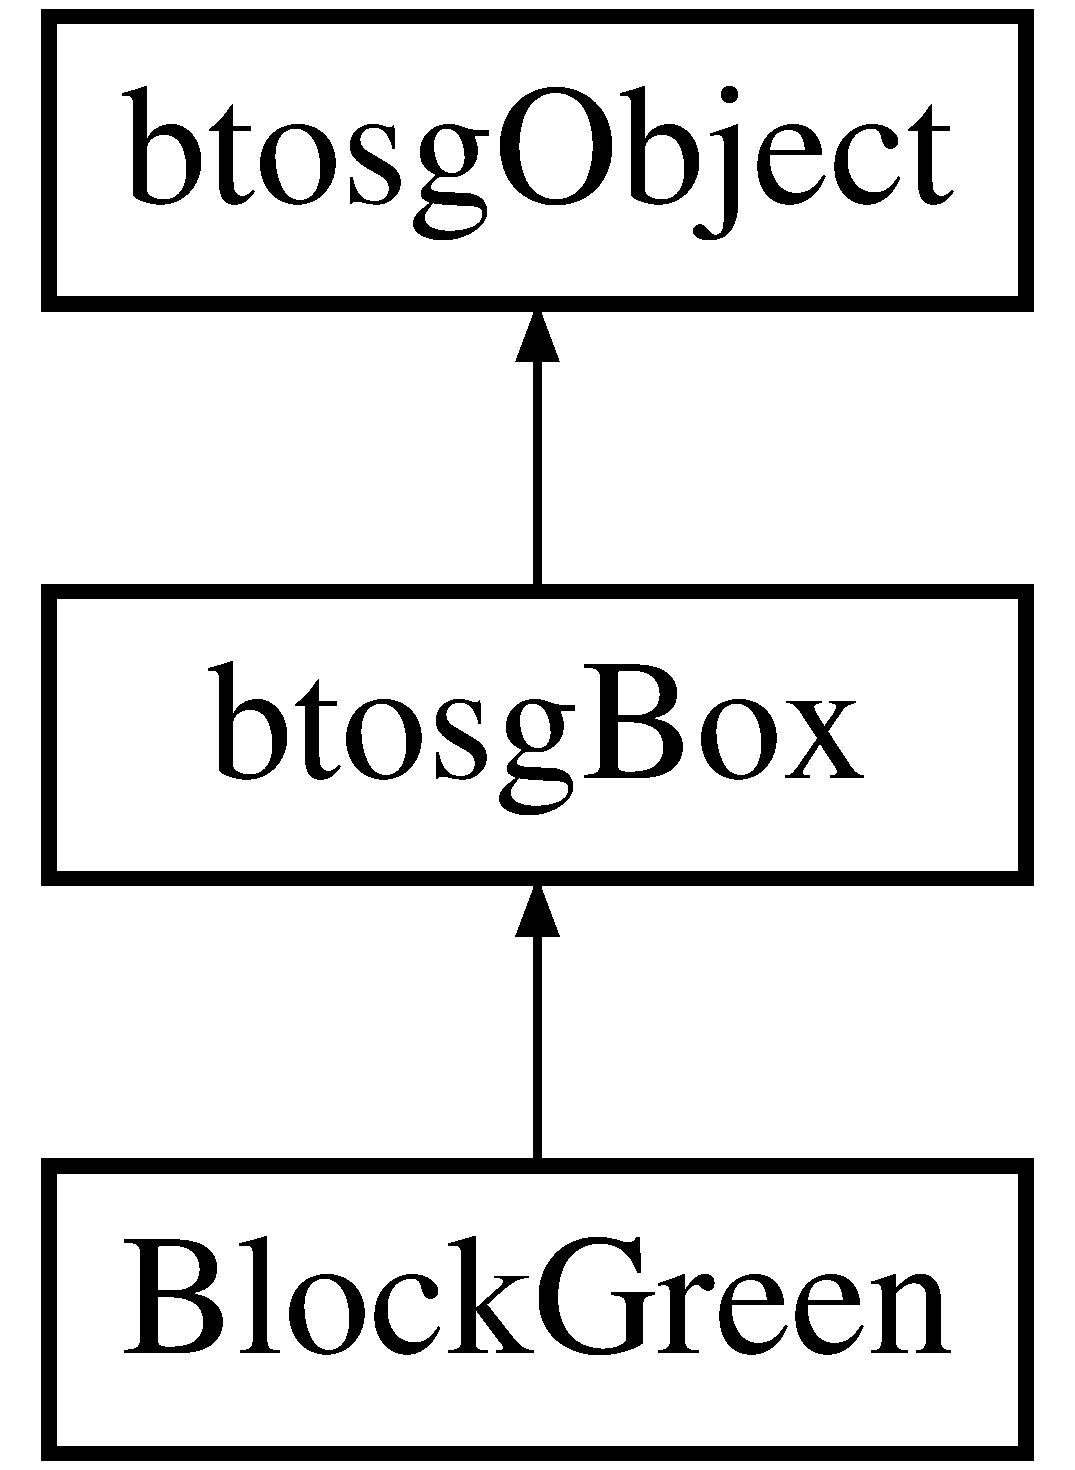
\includegraphics[height=3.000000cm]{classBlockGreen}
\end{center}
\end{figure}
\subsection*{Public Member Functions}
\begin{DoxyCompactItemize}
\item 
\mbox{\Hypertarget{classBlockGreen_aa1ce13416cb41b01defc2291a1627fd4}\label{classBlockGreen_aa1ce13416cb41b01defc2291a1627fd4}} 
{\bfseries Block\+Green} (float x, float y, float z)
\item 
\mbox{\Hypertarget{classBlockGreen_a4e29c2c2494b8237fa4431f47ada23c9}\label{classBlockGreen_a4e29c2c2494b8237fa4431f47ada23c9}} 
{\bfseries Block\+Green} (float x, float z)
\end{DoxyCompactItemize}
\subsection*{Additional Inherited Members}


The documentation for this class was generated from the following file\+:\begin{DoxyCompactItemize}
\item 
car.\+cpp\end{DoxyCompactItemize}

\hypertarget{classBlockRed}{}\section{Block\+Red Class Reference}
\label{classBlockRed}\index{Block\+Red@{Block\+Red}}
Inheritance diagram for Block\+Red\+:\begin{figure}[H]
\begin{center}
\leavevmode
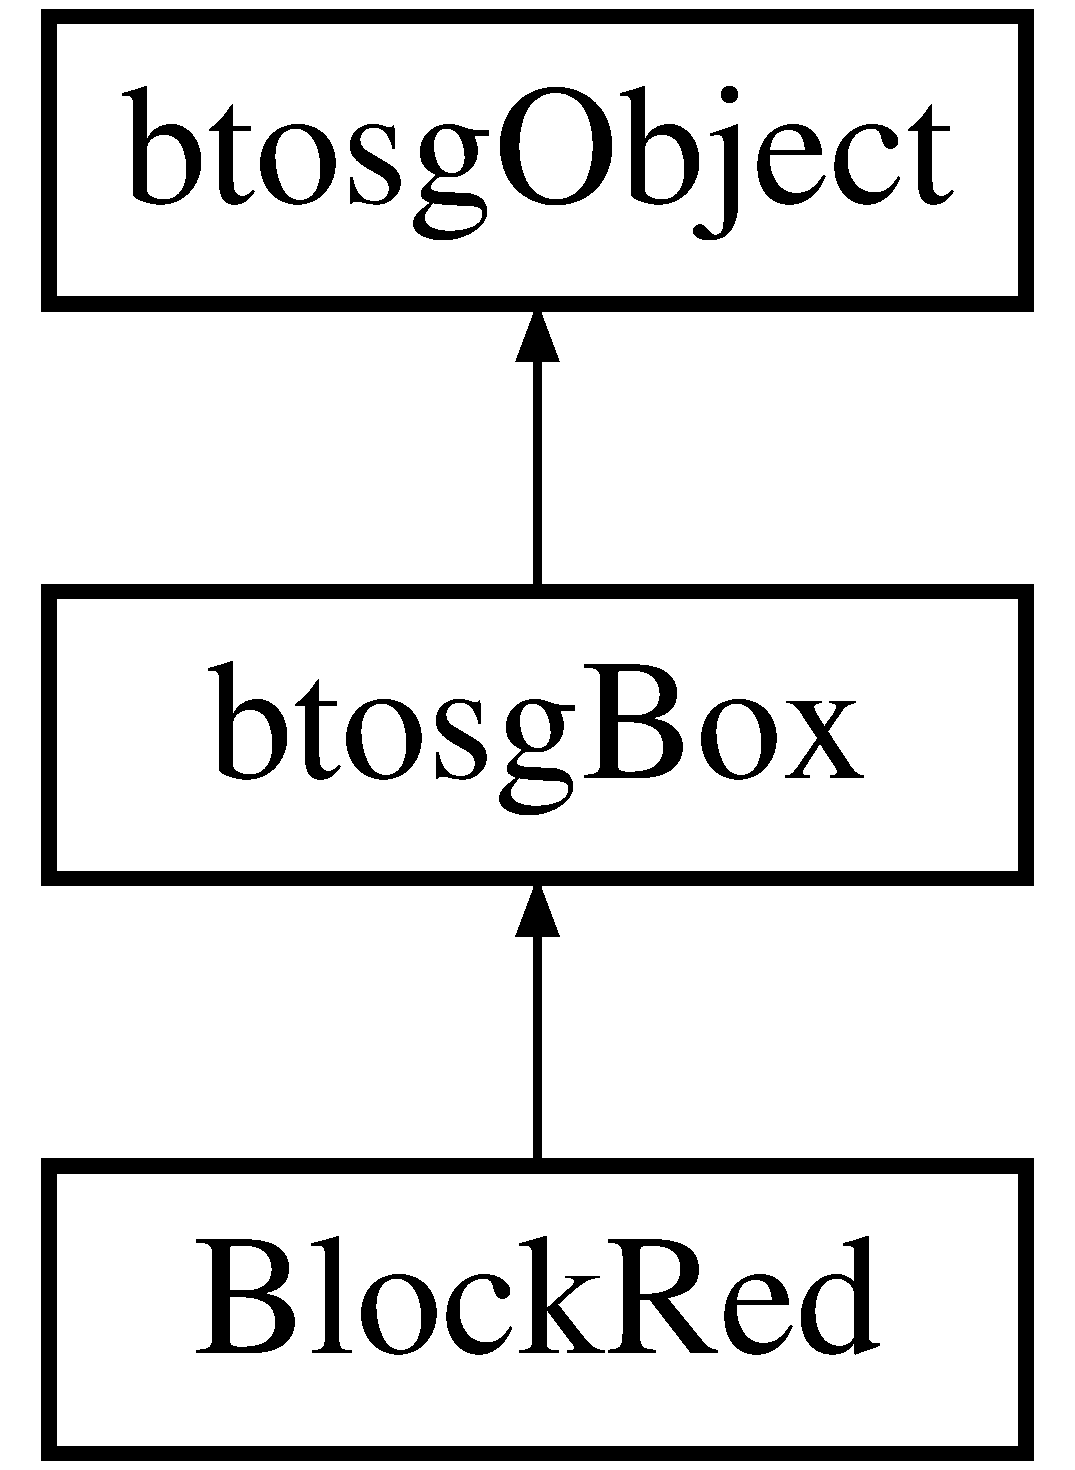
\includegraphics[height=3.000000cm]{classBlockRed}
\end{center}
\end{figure}
\subsection*{Public Member Functions}
\begin{DoxyCompactItemize}
\item 
\mbox{\Hypertarget{classBlockRed_a56631421f23f2dd67a32fe366b2612f2}\label{classBlockRed_a56631421f23f2dd67a32fe366b2612f2}} 
{\bfseries Block\+Red} (float x, float y, float z)
\item 
\mbox{\Hypertarget{classBlockRed_abd643d994ad3cbe6064d7e4703b064d1}\label{classBlockRed_abd643d994ad3cbe6064d7e4703b064d1}} 
{\bfseries Block\+Red} (float x, float z)
\end{DoxyCompactItemize}
\subsection*{Additional Inherited Members}


The documentation for this class was generated from the following file\+:\begin{DoxyCompactItemize}
\item 
car.\+cpp\end{DoxyCompactItemize}

\hypertarget{classbtosgBox}{}\section{btosg\+Box Class Reference}
\label{classbtosgBox}\index{btosg\+Box@{btosg\+Box}}
Inheritance diagram for btosg\+Box\+:\begin{figure}[H]
\begin{center}
\leavevmode
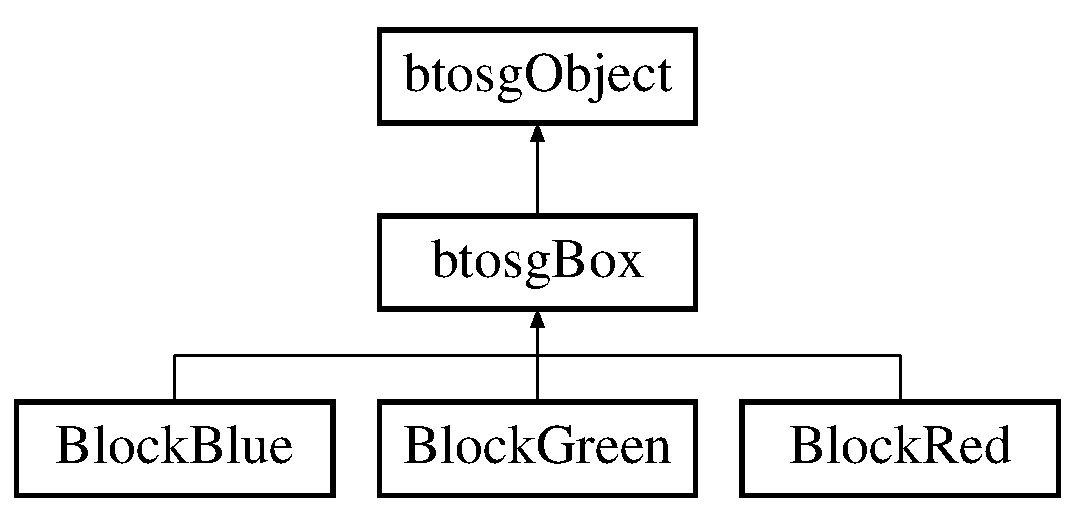
\includegraphics[height=3.000000cm]{classbtosgBox}
\end{center}
\end{figure}
\subsection*{Public Member Functions}
\begin{DoxyCompactItemize}
\item 
\mbox{\Hypertarget{classbtosgBox_a7b899d77d6ce1cd9fd1a506219814c2c}\label{classbtosgBox_a7b899d77d6ce1cd9fd1a506219814c2c}} 
{\bfseries btosg\+Box} (osg\+::\+Vec3 dim=osg\+::\+Vec3(1., 1., 1.), double m=1.)
\item 
\mbox{\Hypertarget{classbtosgBox_a0b7809cf498d50ced7c6e4a1bf0f5470}\label{classbtosgBox_a0b7809cf498d50ced7c6e4a1bf0f5470}} 
{\bfseries btosg\+Box} (float x, float y, float z)
\item 
\mbox{\Hypertarget{classbtosgBox_a3b17e84e3f94aabdc7b8517bd802a5c9}\label{classbtosgBox_a3b17e84e3f94aabdc7b8517bd802a5c9}} 
{\bfseries btosg\+Box} (float r)
\end{DoxyCompactItemize}
\subsection*{Public Attributes}
\begin{DoxyCompactItemize}
\item 
\mbox{\Hypertarget{classbtosgBox_a1d1e4744d9e377e1462ea097dacef716}\label{classbtosgBox_a1d1e4744d9e377e1462ea097dacef716}} 
float {\bfseries dx}
\item 
\mbox{\Hypertarget{classbtosgBox_a7665337187adb52a1ce3b4cf2819217d}\label{classbtosgBox_a7665337187adb52a1ce3b4cf2819217d}} 
float {\bfseries dy}
\item 
\mbox{\Hypertarget{classbtosgBox_a1dd905f6afb684d5d364f2b211dbab97}\label{classbtosgBox_a1dd905f6afb684d5d364f2b211dbab97}} 
float {\bfseries dz}
\end{DoxyCompactItemize}


The documentation for this class was generated from the following file\+:\begin{DoxyCompactItemize}
\item 
btosg.\+h\end{DoxyCompactItemize}

\hypertarget{classbtosgCone}{}\section{btosg\+Cone Class Reference}
\label{classbtosgCone}\index{btosg\+Cone@{btosg\+Cone}}
Inheritance diagram for btosg\+Cone\+:\begin{figure}[H]
\begin{center}
\leavevmode
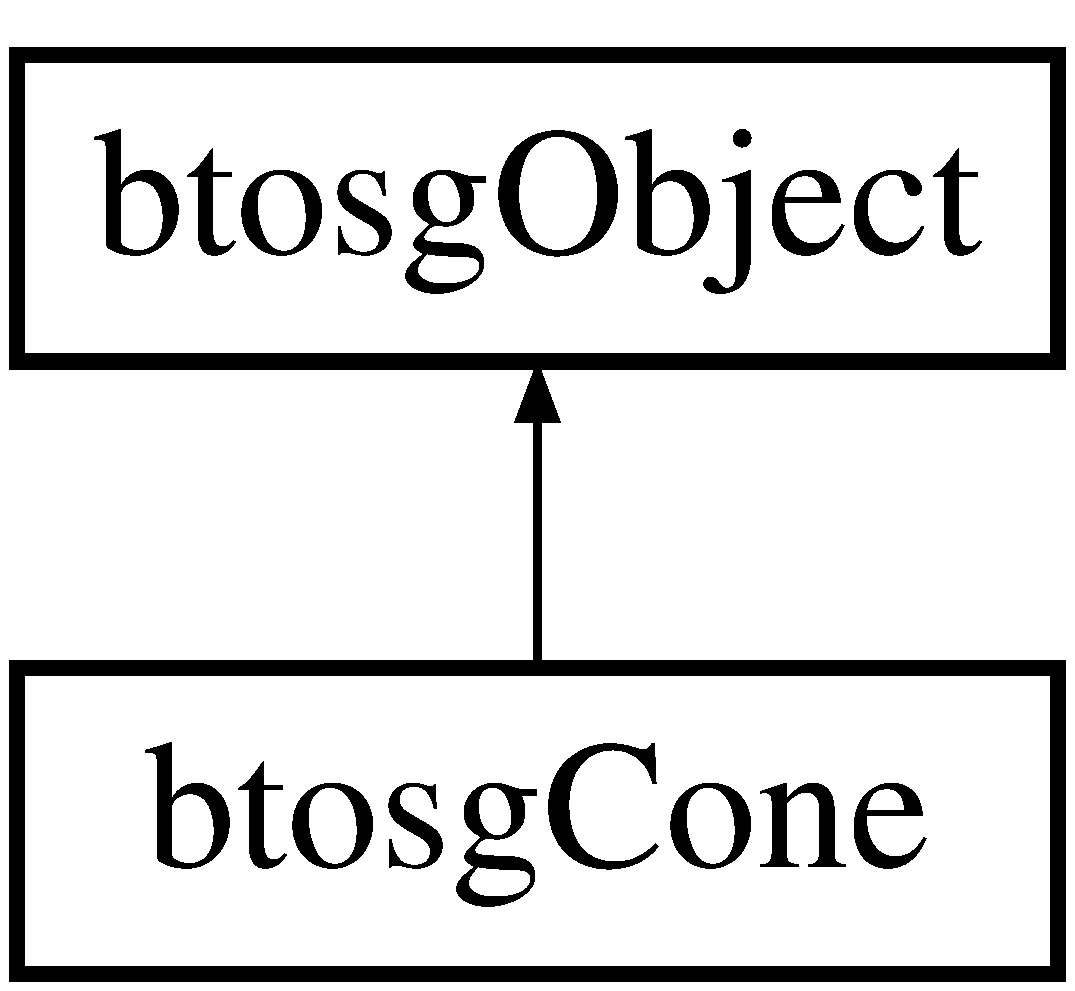
\includegraphics[height=2.000000cm]{classbtosgCone}
\end{center}
\end{figure}
\subsection*{Public Member Functions}
\begin{DoxyCompactItemize}
\item 
\mbox{\Hypertarget{classbtosgCone_a119bf79e2311ba084939d3e25086751c}\label{classbtosgCone_a119bf79e2311ba084939d3e25086751c}} 
{\bfseries btosg\+Cone} (float r=0.\+5, float h=1)
\end{DoxyCompactItemize}
\subsection*{Public Attributes}
\begin{DoxyCompactItemize}
\item 
\mbox{\Hypertarget{classbtosgCone_a75e351e13ad1e4d402f44a36838a6f4a}\label{classbtosgCone_a75e351e13ad1e4d402f44a36838a6f4a}} 
float {\bfseries radius}
\item 
\mbox{\Hypertarget{classbtosgCone_a1ddcbd82ff1fbaf69bc99d242819b83f}\label{classbtosgCone_a1ddcbd82ff1fbaf69bc99d242819b83f}} 
float {\bfseries height}
\end{DoxyCompactItemize}


The documentation for this class was generated from the following file\+:\begin{DoxyCompactItemize}
\item 
btosg.\+h\end{DoxyCompactItemize}

\hypertarget{classbtosgCylinder}{}\section{btosg\+Cylinder Class Reference}
\label{classbtosgCylinder}\index{btosg\+Cylinder@{btosg\+Cylinder}}
Inheritance diagram for btosg\+Cylinder\+:\begin{figure}[H]
\begin{center}
\leavevmode
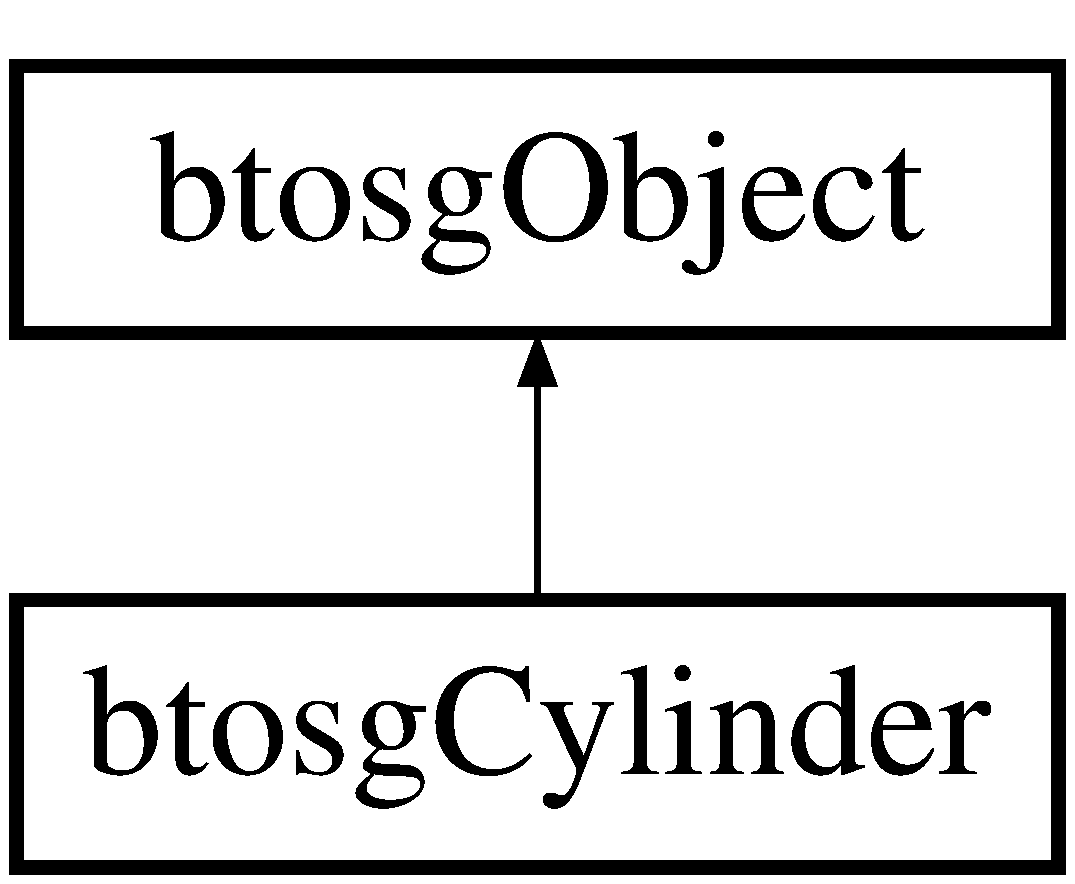
\includegraphics[height=2.000000cm]{classbtosgCylinder}
\end{center}
\end{figure}
\subsection*{Public Member Functions}
\begin{DoxyCompactItemize}
\item 
\mbox{\Hypertarget{classbtosgCylinder_a85e2517d8fd8a16ad7514f2f70cc1086}\label{classbtosgCylinder_a85e2517d8fd8a16ad7514f2f70cc1086}} 
{\bfseries btosg\+Cylinder} (float r=0.\+5, float h=1)
\end{DoxyCompactItemize}
\subsection*{Public Attributes}
\begin{DoxyCompactItemize}
\item 
\mbox{\Hypertarget{classbtosgCylinder_a6589c522ac0b82880287f28e791acac0}\label{classbtosgCylinder_a6589c522ac0b82880287f28e791acac0}} 
float {\bfseries radius}
\item 
\mbox{\Hypertarget{classbtosgCylinder_a4fca9b21b059fdcb762b5e8ce8a3e0eb}\label{classbtosgCylinder_a4fca9b21b059fdcb762b5e8ce8a3e0eb}} 
float {\bfseries height}
\end{DoxyCompactItemize}


The documentation for this class was generated from the following file\+:\begin{DoxyCompactItemize}
\item 
btosg.\+h\end{DoxyCompactItemize}

\hypertarget{classbtosgHUD}{}\section{btosg\+H\+UD Class Reference}
\label{classbtosgHUD}\index{btosg\+H\+UD@{btosg\+H\+UD}}
Inheritance diagram for btosg\+H\+UD\+:\begin{figure}[H]
\begin{center}
\leavevmode
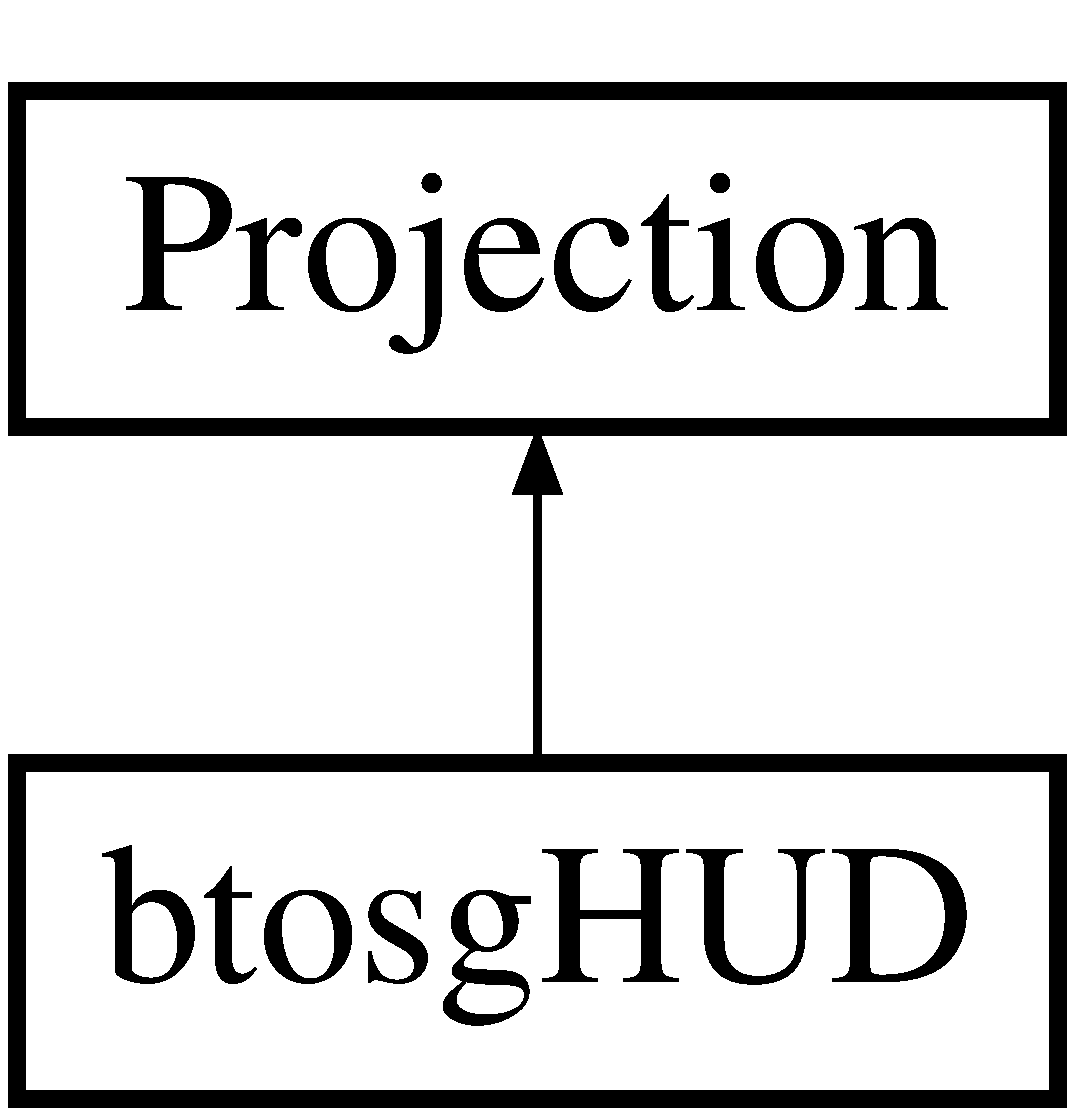
\includegraphics[height=2.000000cm]{classbtosgHUD}
\end{center}
\end{figure}
\subsection*{Public Member Functions}
\begin{DoxyCompactItemize}
\item 
\mbox{\Hypertarget{classbtosgHUD_a18c1eb80934574e6bdabbbee43e0bfeb}\label{classbtosgHUD_a18c1eb80934574e6bdabbbee43e0bfeb}} 
void {\bfseries set\+Background} ()
\item 
\mbox{\Hypertarget{classbtosgHUD_a182be3e4bdf00f9ff2b9c482833089a4}\label{classbtosgHUD_a182be3e4bdf00f9ff2b9c482833089a4}} 
virtual bool {\bfseries add\+Drawable} (osg\+::\+Drawable $\ast$td)
\end{DoxyCompactItemize}


The documentation for this class was generated from the following file\+:\begin{DoxyCompactItemize}
\item 
btosg\+H\+U\+D.\+h\end{DoxyCompactItemize}

\hypertarget{classbtosgObject}{}\section{btosg\+Object Class Reference}
\label{classbtosgObject}\index{btosg\+Object@{btosg\+Object}}
Inheritance diagram for btosg\+Object\+:\begin{figure}[H]
\begin{center}
\leavevmode
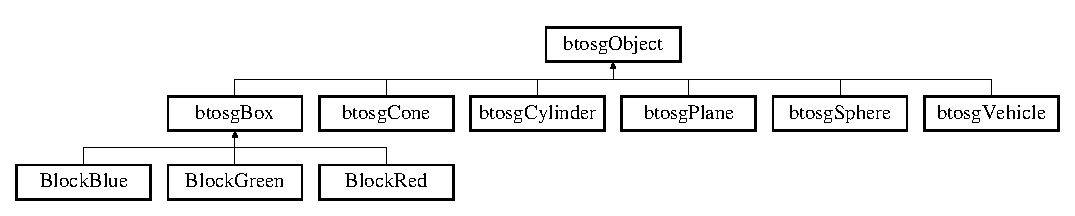
\includegraphics[height=2.448980cm]{classbtosgObject}
\end{center}
\end{figure}
\subsection*{Public Member Functions}
\begin{DoxyCompactItemize}
\item 
\mbox{\Hypertarget{classbtosgObject_ab06a1b3f357209214c6440cd5746523e}\label{classbtosgObject_ab06a1b3f357209214c6440cd5746523e}} 
void {\bfseries set\+Name} (char const $\ast$n)
\item 
\mbox{\Hypertarget{classbtosgObject_a91da93c82d48b86192f0cbb16054fe57}\label{classbtosgObject_a91da93c82d48b86192f0cbb16054fe57}} 
void {\bfseries set\+Mass} (double m)
\item 
\mbox{\Hypertarget{classbtosgObject_a77a1434498d7a6d00c415042a995d119}\label{classbtosgObject_a77a1434498d7a6d00c415042a995d119}} 
bt\+Vector3 {\bfseries get\+Position} ()
\item 
\mbox{\Hypertarget{classbtosgObject_a9cadb03762699412552601196950a039}\label{classbtosgObject_a9cadb03762699412552601196950a039}} 
bt\+Quaternion {\bfseries get\+Rotation} ()
\item 
\mbox{\Hypertarget{classbtosgObject_afef1fe06635566ab9cee134f72439e02}\label{classbtosgObject_afef1fe06635566ab9cee134f72439e02}} 
bt\+Vector3 {\bfseries get\+Euler} ()
\item 
\mbox{\Hypertarget{classbtosgObject_ad0f76df8e8bde6c8a9d1b1d53551172b}\label{classbtosgObject_ad0f76df8e8bde6c8a9d1b1d53551172b}} 
void {\bfseries set\+Position} (const bt\+Vector3 \&p)
\item 
\mbox{\Hypertarget{classbtosgObject_adb9f2cff0faf66dc252cd7c97b11ac84}\label{classbtosgObject_adb9f2cff0faf66dc252cd7c97b11ac84}} 
void {\bfseries set\+Position} (float x, float y, float z)
\item 
\mbox{\Hypertarget{classbtosgObject_a656412794a971a10478aedb520f298bf}\label{classbtosgObject_a656412794a971a10478aedb520f298bf}} 
void {\bfseries set\+Rotation} (bt\+Quaternion q)
\item 
\mbox{\Hypertarget{classbtosgObject_a4d21ca59b944fd26644db35d3e9ba67a}\label{classbtosgObject_a4d21ca59b944fd26644db35d3e9ba67a}} 
void {\bfseries set\+Rotation} (float x, float y, float z, float w)
\item 
\mbox{\Hypertarget{classbtosgObject_ae803e0566f0d7b3ffca686b968b297f8}\label{classbtosgObject_ae803e0566f0d7b3ffca686b968b297f8}} 
void {\bfseries set\+Rotation} (osg\+::\+Quat q)
\item 
\mbox{\Hypertarget{classbtosgObject_aff54acbc7c66811efb0cf2838107a241}\label{classbtosgObject_aff54acbc7c66811efb0cf2838107a241}} 
void {\bfseries set\+Texture} (char const $\ast$fname)
\item 
\mbox{\Hypertarget{classbtosgObject_a6ab7b9e0553dab398b980637788b56a8}\label{classbtosgObject_a6ab7b9e0553dab398b980637788b56a8}} 
void {\bfseries set\+Material} (osg\+::ref\+\_\+ptr$<$ osg\+::\+Material $>$ mat)
\item 
\mbox{\Hypertarget{classbtosgObject_acfd70fa6477c80fd7f29ad7ab9f4f067}\label{classbtosgObject_acfd70fa6477c80fd7f29ad7ab9f4f067}} 
void {\bfseries log\+Position} ()
\item 
virtual void \hyperlink{classbtosgObject_a342917817dfde62554f83da8e0d5110b}{update} ()
\item 
void \hyperlink{classbtosgObject_a93983f9180dd0672f8779cf2baa78580}{reset} ()
\item 
\mbox{\Hypertarget{classbtosgObject_ad1508a0ce28cfac83e5f0ff6245f91b5}\label{classbtosgObject_ad1508a0ce28cfac83e5f0ff6245f91b5}} 
void {\bfseries set\+Init\+State} ()
\item 
\mbox{\Hypertarget{classbtosgObject_a6ceb08e59ee95acaaef389ee198d2b56}\label{classbtosgObject_a6ceb08e59ee95acaaef389ee198d2b56}} 
void {\bfseries set\+Init\+State} (bt\+Transform i\+State)
\item 
\mbox{\Hypertarget{classbtosgObject_a029dbe9134fa94e7355799f67fb2cd6d}\label{classbtosgObject_a029dbe9134fa94e7355799f67fb2cd6d}} 
void {\bfseries create\+Rigid\+Body} ()
\item 
\mbox{\Hypertarget{classbtosgObject_a91838b8235579da178fcc06e6d3d47f3}\label{classbtosgObject_a91838b8235579da178fcc06e6d3d47f3}} 
void {\bfseries load\+Object\+Model} (char const $\ast$fname)
\end{DoxyCompactItemize}
\subsection*{Public Attributes}
\begin{DoxyCompactItemize}
\item 
\mbox{\Hypertarget{classbtosgObject_afd15726e7a214212d6d5815f8ac1ac6c}\label{classbtosgObject_afd15726e7a214212d6d5815f8ac1ac6c}} 
osg\+::ref\+\_\+ptr$<$ osg\+::\+Position\+Attitude\+Transform $>$ \hyperlink{classbtosgObject_afd15726e7a214212d6d5815f8ac1ac6c}{model}
\begin{DoxyCompactList}\small\item\em Object\textquotesingle{}s graphical model. \end{DoxyCompactList}\item 
\mbox{\Hypertarget{classbtosgObject_a12396e1362797a75473a2e833b579cc9}\label{classbtosgObject_a12396e1362797a75473a2e833b579cc9}} 
char $\ast$ \hyperlink{classbtosgObject_a12396e1362797a75473a2e833b579cc9}{name}
\begin{DoxyCompactList}\small\item\em Object name. \end{DoxyCompactList}\item 
\mbox{\Hypertarget{classbtosgObject_a2dee023f311114e200df9b04c8c1b400}\label{classbtosgObject_a2dee023f311114e200df9b04c8c1b400}} 
bt\+Transform \hyperlink{classbtosgObject_a2dee023f311114e200df9b04c8c1b400}{init\+\_\+state}
\begin{DoxyCompactList}\small\item\em Inital state. Applied on reset events. \end{DoxyCompactList}\item 
\mbox{\Hypertarget{classbtosgObject_a64ccde0543c184ed1749fdb9c9699785}\label{classbtosgObject_a64ccde0543c184ed1749fdb9c9699785}} 
bt\+Rigid\+Body $\ast$ \hyperlink{classbtosgObject_a64ccde0543c184ed1749fdb9c9699785}{body}
\begin{DoxyCompactList}\small\item\em object\textquotesingle{}s rigid body \end{DoxyCompactList}\item 
\mbox{\Hypertarget{classbtosgObject_a0f6a8da01cf643c321bffe86e42604b0}\label{classbtosgObject_a0f6a8da01cf643c321bffe86e42604b0}} 
bt\+Collision\+Shape $\ast$ \hyperlink{classbtosgObject_a0f6a8da01cf643c321bffe86e42604b0}{shape}
\begin{DoxyCompactList}\small\item\em Object\textquotesingle{}s colision shape. \end{DoxyCompactList}\item 
\mbox{\Hypertarget{classbtosgObject_a2418bb2194d5e9b0f1c51c84672ba7d1}\label{classbtosgObject_a2418bb2194d5e9b0f1c51c84672ba7d1}} 
float \hyperlink{classbtosgObject_a2418bb2194d5e9b0f1c51c84672ba7d1}{mass}
\begin{DoxyCompactList}\small\item\em Mass of object. \end{DoxyCompactList}\end{DoxyCompactItemize}


\subsection{Member Function Documentation}
\mbox{\Hypertarget{classbtosgObject_a93983f9180dd0672f8779cf2baa78580}\label{classbtosgObject_a93983f9180dd0672f8779cf2baa78580}} 
\index{btosg\+Object@{btosg\+Object}!reset@{reset}}
\index{reset@{reset}!btosg\+Object@{btosg\+Object}}
\subsubsection{\texorpdfstring{reset()}{reset()}}
{\footnotesize\ttfamily void btosg\+Object\+::reset (\begin{DoxyParamCaption}{ }\end{DoxyParamCaption})\hspace{0.3cm}{\ttfamily [inline]}}

$<$ Reposition object to its inital state. \mbox{\Hypertarget{classbtosgObject_a342917817dfde62554f83da8e0d5110b}\label{classbtosgObject_a342917817dfde62554f83da8e0d5110b}} 
\index{btosg\+Object@{btosg\+Object}!update@{update}}
\index{update@{update}!btosg\+Object@{btosg\+Object}}
\subsubsection{\texorpdfstring{update()}{update()}}
{\footnotesize\ttfamily virtual void btosg\+Object\+::update (\begin{DoxyParamCaption}{ }\end{DoxyParamCaption})\hspace{0.3cm}{\ttfamily [inline]}, {\ttfamily [virtual]}}

$<$ Objects\textquotesingle{}s update callback. This fucntion is called automatically from World\+::setp\+Simulation() for each registered object. Positions graphical object from its physhical state. 

The documentation for this class was generated from the following files\+:\begin{DoxyCompactItemize}
\item 
btosg.\+h\item 
btosg.\+cpp\end{DoxyCompactItemize}

\hypertarget{classbtosgPlane}{}\section{btosg\+Plane Class Reference}
\label{classbtosgPlane}\index{btosg\+Plane@{btosg\+Plane}}
Inheritance diagram for btosg\+Plane\+:\begin{figure}[H]
\begin{center}
\leavevmode
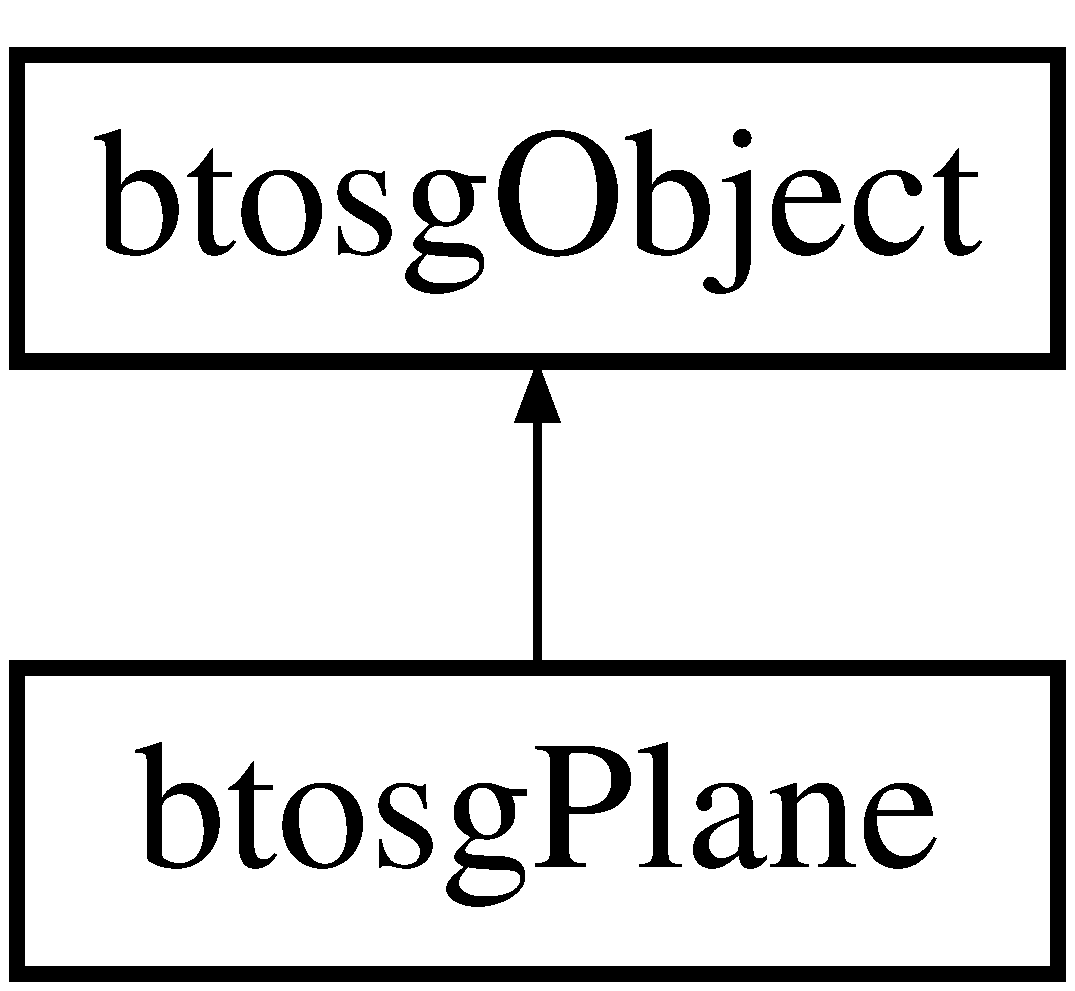
\includegraphics[height=2.000000cm]{classbtosgPlane}
\end{center}
\end{figure}
\subsection*{Public Member Functions}
\begin{DoxyCompactItemize}
\item 
\mbox{\Hypertarget{classbtosgPlane_a4bc8b74d62426eb5fa66355b71569db2}\label{classbtosgPlane_a4bc8b74d62426eb5fa66355b71569db2}} 
{\bfseries btosg\+Plane} (osg\+::\+Vec3 v)
\item 
\mbox{\Hypertarget{classbtosgPlane_a295ebe4cb55a2786764c7840d10895f4}\label{classbtosgPlane_a295ebe4cb55a2786764c7840d10895f4}} 
{\bfseries btosg\+Plane} (float dx, float dy, float dz)
\item 
\mbox{\Hypertarget{classbtosgPlane_a0e6812c186ed1fa128dccf7cd2e525a6}\label{classbtosgPlane_a0e6812c186ed1fa128dccf7cd2e525a6}} 
void {\bfseries create\+Rigid\+Body} ()
\end{DoxyCompactItemize}
\subsection*{Public Attributes}
\begin{DoxyCompactItemize}
\item 
\mbox{\Hypertarget{classbtosgPlane_aca9dda4e87ee5c0d01d45fa8e120e565}\label{classbtosgPlane_aca9dda4e87ee5c0d01d45fa8e120e565}} 
float {\bfseries dx}
\item 
\mbox{\Hypertarget{classbtosgPlane_af3da7fce7bd8792c71c35de95cb8e7cb}\label{classbtosgPlane_af3da7fce7bd8792c71c35de95cb8e7cb}} 
float {\bfseries dy}
\item 
\mbox{\Hypertarget{classbtosgPlane_a87b392e258597ce4ce7c930aa58e99ec}\label{classbtosgPlane_a87b392e258597ce4ce7c930aa58e99ec}} 
float {\bfseries dz}
\end{DoxyCompactItemize}


The documentation for this class was generated from the following file\+:\begin{DoxyCompactItemize}
\item 
btosg.\+h\end{DoxyCompactItemize}

\hypertarget{classbtosgSphere}{}\section{btosg\+Sphere Class Reference}
\label{classbtosgSphere}\index{btosg\+Sphere@{btosg\+Sphere}}
Inheritance diagram for btosg\+Sphere\+:\begin{figure}[H]
\begin{center}
\leavevmode
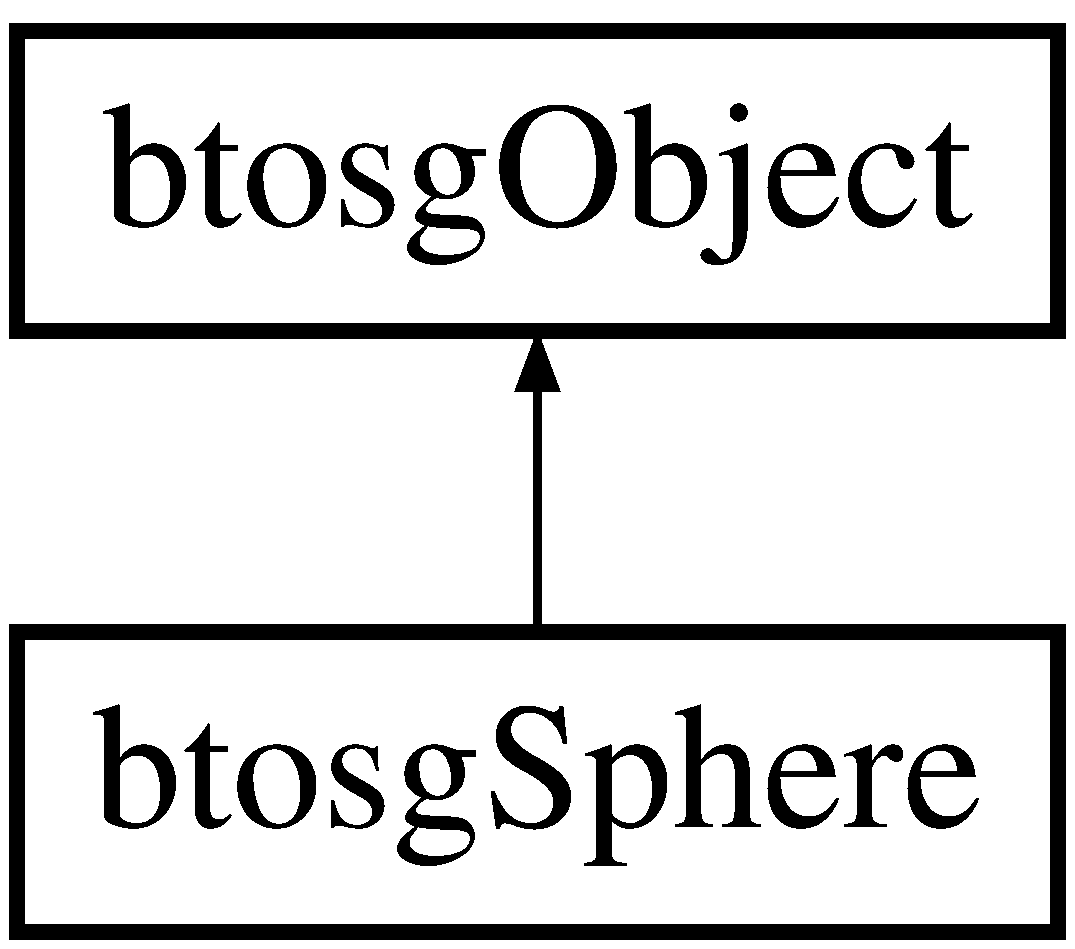
\includegraphics[height=2.000000cm]{classbtosgSphere}
\end{center}
\end{figure}
\subsection*{Public Member Functions}
\begin{DoxyCompactItemize}
\item 
\mbox{\Hypertarget{classbtosgSphere_a39cc5391405e85edcef16200b52e905c}\label{classbtosgSphere_a39cc5391405e85edcef16200b52e905c}} 
{\bfseries btosg\+Sphere} (float r)
\end{DoxyCompactItemize}
\subsection*{Public Attributes}
\begin{DoxyCompactItemize}
\item 
\mbox{\Hypertarget{classbtosgSphere_afd570c85e9ce1b15b2b4b378e4f6abeb}\label{classbtosgSphere_afd570c85e9ce1b15b2b4b378e4f6abeb}} 
float {\bfseries radius}
\end{DoxyCompactItemize}


The documentation for this class was generated from the following file\+:\begin{DoxyCompactItemize}
\item 
btosg.\+h\end{DoxyCompactItemize}

\hypertarget{classbtosgVehicle}{}\section{btosg\+Vehicle Class Reference}
\label{classbtosgVehicle}\index{btosg\+Vehicle@{btosg\+Vehicle}}
Inheritance diagram for btosg\+Vehicle\+:\begin{figure}[H]
\begin{center}
\leavevmode
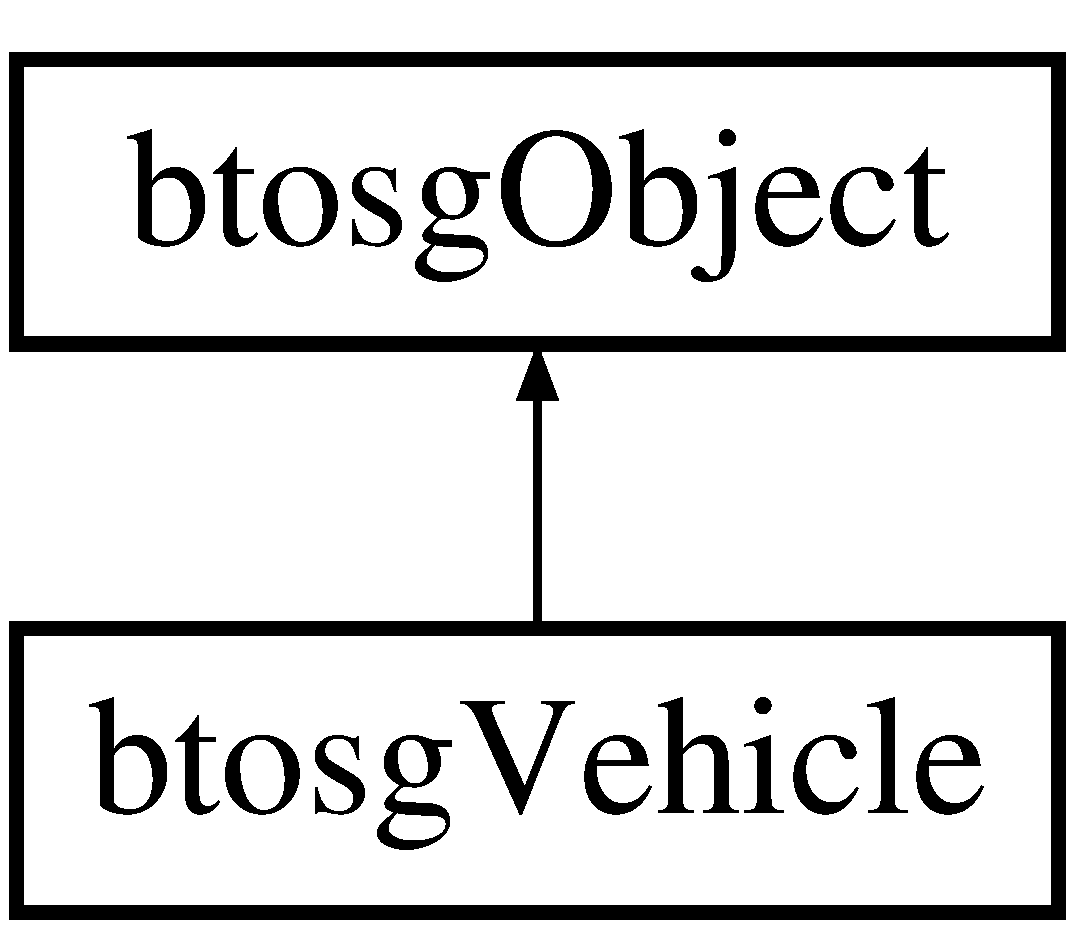
\includegraphics[height=2.000000cm]{classbtosgVehicle}
\end{center}
\end{figure}
\subsection*{Public Member Functions}
\begin{DoxyCompactItemize}
\item 
\mbox{\Hypertarget{classbtosgVehicle_a462222cde5a3480b8964b582fcbf39a3}\label{classbtosgVehicle_a462222cde5a3480b8964b582fcbf39a3}} 
{\bfseries btosg\+Vehicle} (\hyperlink{classbtosgWorld}{btosg\+World} $\ast$world, osg\+::\+Vec3 dim\+Local=osg\+::\+Vec3(2., 0.\+4, 4.), double m=1000.)
\item 
\mbox{\Hypertarget{classbtosgVehicle_a98971fb952c08cb72341a0c333fc66de}\label{classbtosgVehicle_a98971fb952c08cb72341a0c333fc66de}} 
void {\bfseries add\+Wheels} (bt\+Vector3 $\ast$half\+Extents, bt\+Raycast\+Vehicle $\ast$vehicle, bt\+Raycast\+Vehicle\+::bt\+Vehicle\+Tuning tuning)
\item 
\mbox{\Hypertarget{classbtosgVehicle_abe98f64f0a8f37c7c0b244e3afbbcb15}\label{classbtosgVehicle_abe98f64f0a8f37c7c0b244e3afbbcb15}} 
void {\bfseries print\+Info} ()
\item 
\mbox{\Hypertarget{classbtosgVehicle_ae9168c62263b26f95d068d94d6a7cab7}\label{classbtosgVehicle_ae9168c62263b26f95d068d94d6a7cab7}} 
void {\bfseries log\+Position} ()
\item 
\mbox{\Hypertarget{classbtosgVehicle_a5fd0f471df492ac232c9b772a28bd2b9}\label{classbtosgVehicle_a5fd0f471df492ac232c9b772a28bd2b9}} 
virtual void {\bfseries update} ()
\end{DoxyCompactItemize}
\subsection*{Public Attributes}
\begin{DoxyCompactItemize}
\item 
\mbox{\Hypertarget{classbtosgVehicle_aed23010bba3c34158abd4548328b3819}\label{classbtosgVehicle_aed23010bba3c34158abd4548328b3819}} 
float {\bfseries dx}
\item 
\mbox{\Hypertarget{classbtosgVehicle_ae124e1cd8c424080d7be7c47edb07eb1}\label{classbtosgVehicle_ae124e1cd8c424080d7be7c47edb07eb1}} 
float {\bfseries dy}
\item 
\mbox{\Hypertarget{classbtosgVehicle_a39857392dc4882886964c1beefa46268}\label{classbtosgVehicle_a39857392dc4882886964c1beefa46268}} 
float {\bfseries dz}
\item 
\mbox{\Hypertarget{classbtosgVehicle_afed9fb742c4a8ed58e8d6202dfc20344}\label{classbtosgVehicle_afed9fb742c4a8ed58e8d6202dfc20344}} 
osg\+::\+Vec3 {\bfseries dim}
\item 
\mbox{\Hypertarget{classbtosgVehicle_a8f68a9e001e79f61602427228c97fe26}\label{classbtosgVehicle_a8f68a9e001e79f61602427228c97fe26}} 
osg\+::\+Vec3 {\bfseries up}
\item 
\mbox{\Hypertarget{classbtosgVehicle_a5b21a5ad3a8583f773bce6b894ac010d}\label{classbtosgVehicle_a5b21a5ad3a8583f773bce6b894ac010d}} 
osg\+::\+Vec3 {\bfseries front}
\item 
\mbox{\Hypertarget{classbtosgVehicle_ac45b117f8b523f7040de99639deb7522}\label{classbtosgVehicle_ac45b117f8b523f7040de99639deb7522}} 
bt\+Raycast\+Vehicle $\ast$ {\bfseries vehicle}
\item 
\mbox{\Hypertarget{classbtosgVehicle_a37edb4c28551037829ffd79c7bc315ba}\label{classbtosgVehicle_a37edb4c28551037829ffd79c7bc315ba}} 
osg\+::ref\+\_\+ptr$<$ osg\+::\+Position\+Attitude\+Transform $>$ {\bfseries wheel} \mbox{[}4\mbox{]}
\item 
\mbox{\Hypertarget{classbtosgVehicle_a0a9cd6f2c9b0defc44cd5e2e8d597418}\label{classbtosgVehicle_a0a9cd6f2c9b0defc44cd5e2e8d597418}} 
double {\bfseries wheel\+Rotation} \mbox{[}4\mbox{]}
\end{DoxyCompactItemize}


The documentation for this class was generated from the following file\+:\begin{DoxyCompactItemize}
\item 
btosg\+Vehicle.\+h\end{DoxyCompactItemize}

\hypertarget{classbtosgWorld}{}\section{btosg\+World Class Reference}
\label{classbtosgWorld}\index{btosg\+World@{btosg\+World}}
\subsection*{Public Member Functions}
\begin{DoxyCompactItemize}
\item 
void \hyperlink{classbtosgWorld_afce096686d8f84afd8b8fa3f2dc161b8}{step\+Simulation} (bt\+Scalar time\+Step, int max\+Sub\+Steps)
\item 
void \hyperlink{classbtosgWorld_ae5b71c6319dd420479096a265a1725b7}{add\+Object} (class \hyperlink{classbtosgObject}{btosg\+Object} $\ast$obj)
\item 
void \hyperlink{classbtosgWorld_a6af4d066410a86b44fff5563667ea9a9}{reset} ()
\end{DoxyCompactItemize}
\subsection*{Public Attributes}
\begin{DoxyCompactItemize}
\item 
\mbox{\Hypertarget{classbtosgWorld_ad757a7b3b845142f200d1f2127e5372e}\label{classbtosgWorld_ad757a7b3b845142f200d1f2127e5372e}} 
bt\+Dynamics\+World $\ast$ {\bfseries dynamic}
\item 
\mbox{\Hypertarget{classbtosgWorld_ab6d438f54ccfc18955ea43e87731e008}\label{classbtosgWorld_ab6d438f54ccfc18955ea43e87731e008}} 
osg\+::ref\+\_\+ptr$<$ osg\+::\+Group $>$ {\bfseries scene}
\item 
\mbox{\Hypertarget{classbtosgWorld_ab105aa8c0f8bdbdf323d47b902f6aca0}\label{classbtosgWorld_ab105aa8c0f8bdbdf323d47b902f6aca0}} 
std\+::forward\+\_\+list$<$ class \hyperlink{classbtosgObject}{btosg\+Object} $\ast$ $>$ {\bfseries objects}
\end{DoxyCompactItemize}


\subsection{Member Function Documentation}
\mbox{\Hypertarget{classbtosgWorld_ae5b71c6319dd420479096a265a1725b7}\label{classbtosgWorld_ae5b71c6319dd420479096a265a1725b7}} 
\index{btosg\+World@{btosg\+World}!add\+Object@{add\+Object}}
\index{add\+Object@{add\+Object}!btosg\+World@{btosg\+World}}
\subsubsection{\texorpdfstring{add\+Object()}{addObject()}}
{\footnotesize\ttfamily void btosg\+World\+::add\+Object (\begin{DoxyParamCaption}\item[{class \hyperlink{classbtosgObject}{btosg\+Object} $\ast$}]{obj }\end{DoxyParamCaption})}

Registes the object obj into a simulation world. \mbox{\Hypertarget{classbtosgWorld_a6af4d066410a86b44fff5563667ea9a9}\label{classbtosgWorld_a6af4d066410a86b44fff5563667ea9a9}} 
\index{btosg\+World@{btosg\+World}!reset@{reset}}
\index{reset@{reset}!btosg\+World@{btosg\+World}}
\subsubsection{\texorpdfstring{reset()}{reset()}}
{\footnotesize\ttfamily void btosg\+World\+::reset (\begin{DoxyParamCaption}{ }\end{DoxyParamCaption})}

Reset all registered objects. \mbox{\Hypertarget{classbtosgWorld_afce096686d8f84afd8b8fa3f2dc161b8}\label{classbtosgWorld_afce096686d8f84afd8b8fa3f2dc161b8}} 
\index{btosg\+World@{btosg\+World}!step\+Simulation@{step\+Simulation}}
\index{step\+Simulation@{step\+Simulation}!btosg\+World@{btosg\+World}}
\subsubsection{\texorpdfstring{step\+Simulation()}{stepSimulation()}}
{\footnotesize\ttfamily void btosg\+World\+::step\+Simulation (\begin{DoxyParamCaption}\item[{bt\+Scalar}]{time\+Step,  }\item[{int}]{max\+Sub\+Steps }\end{DoxyParamCaption})}

Performs a simulation step. 

The documentation for this class was generated from the following files\+:\begin{DoxyCompactItemize}
\item 
btosg.\+h\item 
btosg.\+cpp\end{DoxyCompactItemize}

\hypertarget{classEventHandler}{}\section{Event\+Handler Class Reference}
\label{classEventHandler}\index{Event\+Handler@{Event\+Handler}}
Inheritance diagram for Event\+Handler\+:\begin{figure}[H]
\begin{center}
\leavevmode
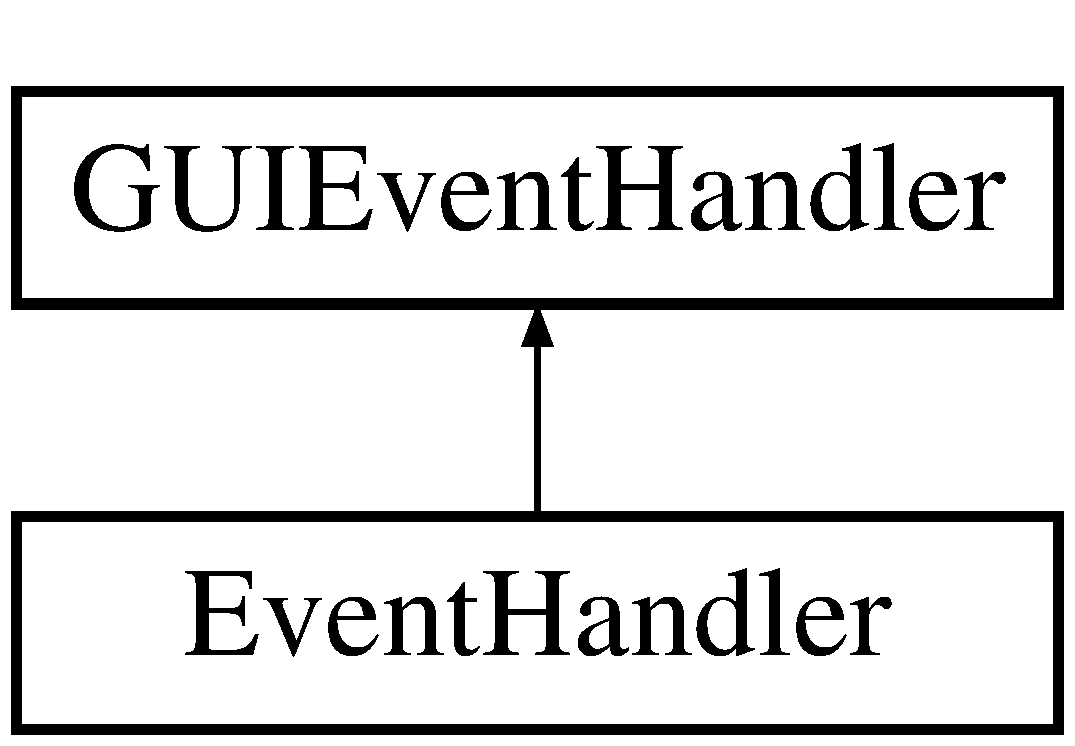
\includegraphics[height=2.000000cm]{classEventHandler}
\end{center}
\end{figure}
\subsection*{Public Member Functions}
\begin{DoxyCompactItemize}
\item 
\mbox{\Hypertarget{classEventHandler_af28f371276fd76929be0a31fbb1be88a}\label{classEventHandler_af28f371276fd76929be0a31fbb1be88a}} 
bool {\bfseries handle} (const osg\+G\+A\+::\+G\+U\+I\+Event\+Adapter \&ea, osg\+G\+A\+::\+G\+U\+I\+Action\+Adapter \&aa)
\end{DoxyCompactItemize}


The documentation for this class was generated from the following file\+:\begin{DoxyCompactItemize}
\item 
car.\+cpp\end{DoxyCompactItemize}

%--- End generated contents ---

% Index
\backmatter
\newpage
\phantomsection
\clearemptydoublepage
\addcontentsline{toc}{chapter}{Index}
\printindex

\end{document}
